% 2018 天津理科第11题：正方体五个面的中心及四棱锥示意图。
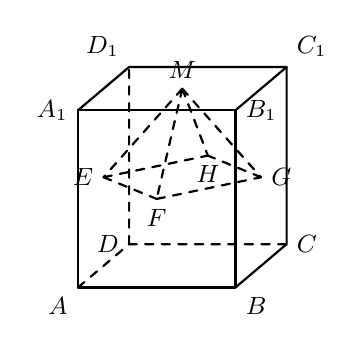
\begin{tikzpicture}[line cap=round,line join=round,thick,every node/.style={font=\small}]
  % Oblique projection of the unit cube; ABCD is the bottom face.
  \coordinate (A) at (0,0);
  \coordinate (B) at (2,0);
  \coordinate (C) at (2.65,.55);
  \coordinate (D) at (.65,.55);
  \coordinate (A1) at (0,2.25);
  \coordinate (B1) at (2,2.25);
  \coordinate (C1) at (2.65,2.8);
  \coordinate (D1) at (.65,2.8);
  % Cube edges: hidden rear-left edges are dashed.
  \draw (A)--(B)--(B1)--(A1)--cycle;
  \draw (A1)--(D1)--(C1)--(B1);
  \draw (B)--(C)--(C1);
  \draw[dashed] (A)--(D)--(C) (D)--(D1);
  % Centers of the top, left, back, right and front faces (ABCD excluded).
  \coordinate (M) at (1.325,2.525);
  \coordinate (E) at (.325,1.4);
  \coordinate (F) at (1,1.125);
  \coordinate (G) at (2.325,1.4);
  \coordinate (H) at (1.65,1.675);
  % The source depicts the internal pyramid construction with dashed lines.
  \draw[dashed] (M)--(E) (M)--(F) (M)--(G) (M)--(H);
  \draw[dashed] (E)--(F) (E)--(H) (F)--(G) (G)--(H);
  \node[below left] at (A) {$A$};
  \node[below right] at (B) {$B$};
  \node[right] at (C) {$C$};
  \node[left] at (D) {$D$};
  \node[left] at (A1) {$A_1$};
  \node[right] at (B1) {$B_1$};
  \node[above right] at (C1) {$C_1$};
  \node[above left] at (D1) {$D_1$};
  \node[above] at (M) {$M$};
  \node[left] at (E) {$E$};
  \node[below] at (F) {$F$};
  \node[right] at (G) {$G$};
  \node[below] at (H) {$H$};
\end{tikzpicture}
